\newif \ifshare
% \sharetrue % Comment this if you want animation
\ifshare % "Share mode" without animation.
\documentclass[table, trans, aspectratio = 169]{beamer}
\else % "Presentation mode" with animation.
\documentclass[table, aspectratio = 169]{beamer}
\fi
\usepackage{default}
\usepackage[T1]{fontenc}
\usepackage[french]{babel}
\usepackage{color}
\usepackage{graphicx}
\usepackage{subfig}
\usepackage{diagbox}


\let\pgfmathMod=\pgfmathmod\relax

\graphicspath{{../figs/PDF/}}

\usetheme{Boadilla}

\definecolor{struct}{HTML}{03a9f4}
\definecolor{alert}{HTML}{f44336}
\definecolor{example}{HTML}{aeea00}
\definecolor{good}{HTML}{8bc34a}
\definecolor{notgoodnotbad}{HTML}{ff9800}

\setbeamercolor{structure}{fg = struct}
\setbeamercolor{normal text}{fg = white, bg = black}
\setbeamercolor{example text}{fg = example}
\setbeamercolor{alerted text}{fg = alert}
\setbeamercolor{footline}{fg = white}

\title[Azure Community Day 2023]{Inspektor Gadget: un Ensemble d'Outils de Débug pour Kubernetes}
\subtitle{Virtual Azure Community Day}
\author[Francis Laniel (\texttt{flaniel@linux.microsoft.com})]{Francis Laniel\\\texttt{flaniel@linux.microsoft.com}}
\date{18 Janvier 2023}

% Custom title page.
\defbeamertemplate*{title page}{customized}[1][]{
	\centering
	\usebeamerfont{title}\usebeamercolor[fg]{title}\inserttitle\par
	\usebeamerfont{subtitle}\usebeamercolor[fg]{subtitle}\insertsubtitle\par
	\bigskip
	\usebeamerfont{author}\usebeamercolor[fg]{normal text}\textbf{\insertauthor}\par
	\bigskip
	\usebeamerfont{date}\usebeamercolor[fg]{normal text}\textbf{\insertdate}\par
	\bigskip
	\bigskip

	\begin{columns}
		\begin{column}{.5\textwidth}
			\centering

			
\includegraphics[scale=2]{microsoft.pdf}
		\end{column}
		\begin{column}{.5\textwidth}
			\centering

			
\includegraphics{kinvolk.pdf}
		\end{column}
	\end{columns}
}

\begin{document}
	% Put these parameters here to avoid compilation error:
	% "! LaTeX Error: Missing \begin{document}."
	% Remove the navigation bar, this is useless...
	\setbeamertemplate{navigation symbols}{}
	% Use square instead of bubbles, see:
	% https://tex.stackexchange.com/a/69721
	\setbeamertemplate{section in toc}[square]
	% Modify the shaded value to 60% instead of 20%, see:
	% https://tex.stackexchange.com/a/66703
	\setbeamertemplate{sections/subsections in toc shaded}[default][50]
	% Use circle instead of bubbles for itemize, see:
	% \setbeamertemplate{itemize items}[circle]
	\setbeamertemplate{itemize items}[square]
	\setbeamertemplate{enumerate items}[square]

	\maketitle

	\section{Introduction}
	\begin{frame}
		\frametitle{Les conteneurs}

		\begin{columns}
			\begin{column}{.5\textwidth}
				Les conteneurs s'appuient sur plusieurs fonctionnalités du noyau :
				\begin{description}
					\item[Les \texttt{namespaces} :] Isolation de sécurité \cite{rami_rosen_namespace_2016, kerrisk_lce_2012, kerrisk_namespaces_2013}.
					\item[Les \texttt{cgroups} :] Isolation de ressources \cite{rami_rosen_namespace_2016, hiroyu_cgroup_2008}.
				\end{description}
			\end{column}
			\begin{column}{.5\textwidth}
				\centering

				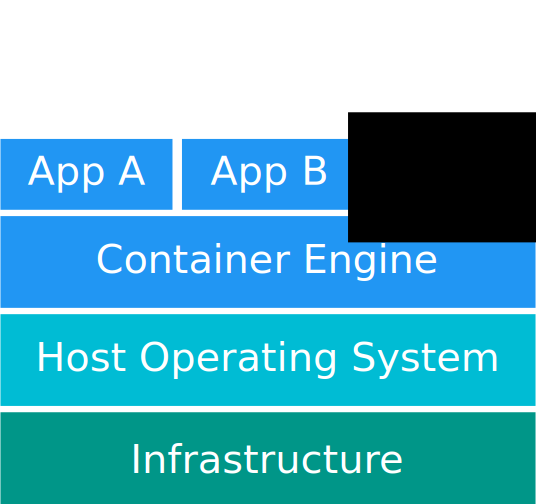
\includegraphics[scale = .42]{container.pdf}

				Container (\texttt{docker}, \texttt{lxc}, \texttt{podman}, etc.)
			\end{column}
		\end{columns}
	\end{frame}

	\begin{frame}
		\frametitle{Kubernetes}

		\begin{columns}
			\begin{column}{.3\textwidth}
				D'après la documentation \cite{kubernetes_developers_quest-ce-que_2022}:
				\begin{quote}
					Kubernetes fournit un environnement de gestion \textbf{focalisé sur le conteneur} [...]. Il orchestre les ressources machines [...].
				\end{quote}
			\end{column}
			\begin{column}{.7\textwidth}
				\centering

				\includegraphics<1>[scale=.33]{k8s-fig1.pdf}%
				\includegraphics<2>[scale=.33]{k8s-fig2.pdf}%
				\includegraphics<3>[scale=.33]{k8s-fig3.pdf}%
				\includegraphics<4>[scale=.33]{k8s-fig4.pdf}%
				\includegraphics<5>[scale=.33]{k8s-fig5.pdf}%

				Architecture interne de Kubernetes
			\end{column}
		\end{columns}
	\end{frame}

	\begin{frame}
		\frametitle{Le \textit{cloud}}
		\framesubtitle{Introduction}

		Le \textit{cloud} consiste en \cite{amazon_quest_ce_nodate} :
		\begin{quote}
			[...] la mise à disposition de ressources informatiques à la demande via Internet, avec une tarification en fonction de votre utilisation.
		\end{quote}

		\bigskip

		\onslide<2->{
			Pour le client, il permet \cite{amazon_quest_ce_nodate} :
			\begin{itemize}
				\item L'agilité
				\item L'élasticité
				\item La réduction des coûts
				\item Le déploiement mondiale en quelques instants
			\end{itemize}
		}

		\bigskip

		\onslide<3>{
			Kubernetes peut pleinement s'exprimer grâce à la mise à disposition de ressources informatiques permise par le cloud.

			Il devient notamment très facile d'ajouter ou de retirer dynamiquement des nœuds.

			Ainsi, de nombreux fournisseurs de services \textit{cloud} proposent d'héberger des clusters Kubernetes \cite{azure_developers_service_nodate, amazon_developers_amazon_nodate}.
		}
	\end{frame}

	\section{Problème}
	\begin{frame}
		\frametitle{Problèmes pour débuger}

		L'utilisation de Kubernetes dans le cloud pose plusieurs problèmes pour débuger, entre autres:
		\begin{itemize}
			\item L'application ne s'exécute plus localement.
			\item Il faut prendre en compte les communications entre les différents \textit{pods}.
		\end{itemize}
	\end{frame}

	\section{Inspektor Gadget}
	\begin{frame}
		\frametitle{Inspektor Gadget}
		\framesubtitle{Présentation}

		\begin{columns}
			\begin{column}{.3\textwidth}
				\centering

				
\includegraphics[scale=.33]{inspektor_gadget.pdf}%

				Un couteau suisse basé sur eBPF \cite{inspektor_gadget_contributors_inspektor_nodate}.
			\end{column}
			\begin{column}{.7\textwidth}
				\centering

				\includegraphics<1>[scale=.2]{inspektor_gadget_tools-fig1.pdf}%
				\includegraphics<2>[scale=.2]{inspektor_gadget_tools-fig2.pdf}%
				\includegraphics<3>[scale=.2]{inspektor_gadget_tools-fig3.pdf}%
				\includegraphics<4>[scale=.2]{inspektor_gadget_tools-fig4.pdf}%
				\includegraphics<5>[scale=.2]{inspektor_gadget_tools-fig5.pdf}%
				\includegraphics<6>[scale=.2]{inspektor_gadget_tools-fig6.pdf}%

				Les différents outils fournis par Inspektor Gadget.
			\end{column}
		\end{columns}
	\end{frame}

	\begin{frame}
		\frametitle{Inspektor Gadget}
		\framesubtitle{Démonstrations simples}

		\begin{enumerate}
			\item Tracer la création de nouveau processus avec \texttt{kubectl gadget trace exec}.
			\item \texttt{kubectl gadget snapshot process} comparé à \texttt{kubectl exec pod-name ---- ps}.
		\end{enumerate}
	\end{frame}

	\begin{frame}
		\frametitle{Inspektor Gadget}
		\framesubtitle{Qu'est-ce que la fonctionnalité eBPF ?}

		D'après Brendan Gregg \cite{gregg_learn_2019}:
		\begin{quote}
			eBPF does to Linux what JavaScript does to HTML.
			[...]
			[W]ith eBPF, instead of a fixed kernel, you can now write mini programs that run on events like disk I/O, which are run in a safe virtual machine in the kernel.
		\end{quote}

		\bigskip

		\onslide<2>{
			La surêté des programmes eBPF vient toutefois avec certaines limitations, entre autres:
			\begin{itemize}
				\item Il n'est pas possible d'écrire du code eBPF comprenant une boucle infinie ou une boucle qui ne soit pas statiquement bornée.
				\item Il n'existe pas de fonction analogue à \texttt{malloc} en eBPF.
			\end{itemize}
		}
	\end{frame}

	\begin{frame}
		\frametitle{Inspektor Gadget}
		\framesubtitle{eBPF dans le noyau Linux}

		\centering

		\includegraphics<1>[scale=.5]{kernel_ebpf-fig1.pdf}%
		\includegraphics<2>[scale=.5]{kernel_ebpf-fig2.pdf}%
		\includegraphics<3>[scale=.5]{kernel_ebpf-fig3.pdf}%
		\includegraphics<4>[scale=.5]{kernel_ebpf-fig4.pdf}%

		Développement, chargement et exécution d'un programme eBPF \cite{ebpf_contributors_what_nodate}.
	\end{frame}

	\begin{frame}
		\frametitle{Inspektor Gadget}
		\framesubtitle{Architecture interne}

		\centering

		\includegraphics<1>[scale=.5]{gadget_tracer_manager-fig1.pdf}%
		\includegraphics<2>[scale=.5]{gadget_tracer_manager-fig2.pdf}%
		\includegraphics<3>[scale=.5]{gadget_tracer_manager-fig3.pdf}%
		\includegraphics<4>[scale=.5]{gadget_tracer_manager-fig4.pdf}%
		\includegraphics<5>[scale=.5]{gadget_tracer_manager-fig5.pdf}%
	\end{frame}

	\begin{frame}
		\frametitle{Inspektor Gadget}
		\framesubtitle{Connexion à Kubernetes}

		\centering

		\includegraphics<1>[scale=.5]{inspektor_gadget_k8s-fig1.pdf}%
		\includegraphics<2>[scale=.5]{inspektor_gadget_k8s-fig2.pdf}%
		\includegraphics<3>[scale=.5]{inspektor_gadget_k8s-fig3.pdf}%
		\includegraphics<4>[scale=.5]{inspektor_gadget_k8s-fig4.pdf}%
		\includegraphics<5>[scale=.5]{inspektor_gadget_k8s-fig5.pdf}%
		\includegraphics<6>[scale=.5]{inspektor_gadget_k8s-fig6.pdf}%
		\includegraphics<7>[scale=.5]{inspektor_gadget_k8s-fig7.pdf}%
		\includegraphics<8>[scale=.5]{inspektor_gadget_k8s-fig8.pdf}%
		\includegraphics<9>[scale=.5]{inspektor_gadget_k8s-fig9.pdf}%
	\end{frame}

	\begin{frame}
		\frametitle{Inspektor Gadget}
		\framesubtitle{Démonstration complète}

		Comment utiliser Inspektor Gadget pour vérifier les \textit{capabilities} accordées à un conteneur ?
	\end{frame}

	\section{Conclusion}
	\begin{frame}
		\frametitle{Conclusion et travaux futurs}

		Conclusion:
		\begin{enumerate}
			\item Inspektor Gadget permet de monitorer des applications conteneurisées.
			\item Il offre ainsi une aide précieuse pour débuger ces applications.
		\end{enumerate}

		\bigskip

		\onslide<2->{
			Travaux futurs:
			\begin{enumerate}
				\item Amélioration du passage à l'échelle.
				\item Ajout de nouveaux gadgets.
			\end{enumerate}
		}
	\end{frame}

	\begin{frame}[allowframebreaks, noframenumbering]
		\frametitle{Bibliographie}
		\setbeamertemplate{bibliography item}[text]

		\begin{scriptsize}
			\bibliographystyle{IEEEtran}
			\bibliography{beamer}
		\end{scriptsize}
	\end{frame}
\end{document}
